\chapter{Análisis de las herramientas seleccionadas \label{propuesta}}


\section{Docker\label{Docker}}


Docker es un proyecto OpenSource que nos ayudará, de una forma eficiente,
simple, segura, portable y replicable a lanzar servicios
\cite{Dck-5,Dck-6}. Para entender Docker, debemos entender el concepto de
contenedor. Según la definición que nos da RedHat, un contenedor es:

\begin{quote}

  \small ``Un contenedor de Linux es un conjunto de procesos que están
  separados del resto del sistema, que se pueden ejecutar desde una imagen
  diferente que proporciona todos los archivos necesarios para dar soporte
  a los procesos. Al proporcionar una imagen que contiene todas las
  dependencias de una aplicación, es portátil y consistente mientras cambia
  de la etapa de desarrollo a la de prueba y, finalmente, a la de
  producción.''\cite{Dck-7}

\end{quote}

En definitiva, un contenedor, a diferencia de una máquina virtual, no tiene
que usar la capa del sistema operativo y esto hace que tampoco necesite el
{\em hypervisor}. Por tanto, un contenedor es capaz de lanzar diferentes
aplicaciones y librerías sobre la capa del sistema operativo que las aloja
de una forma aislada y segura permitiendo, además, un arranque mucho más
rápido, ya que no tiene que cargar la imagen del SO. Esto lo podemos ver en
la figura \ref{dock-1} \cite{Dck-7}.

\begin{figure}[htp]
\centering
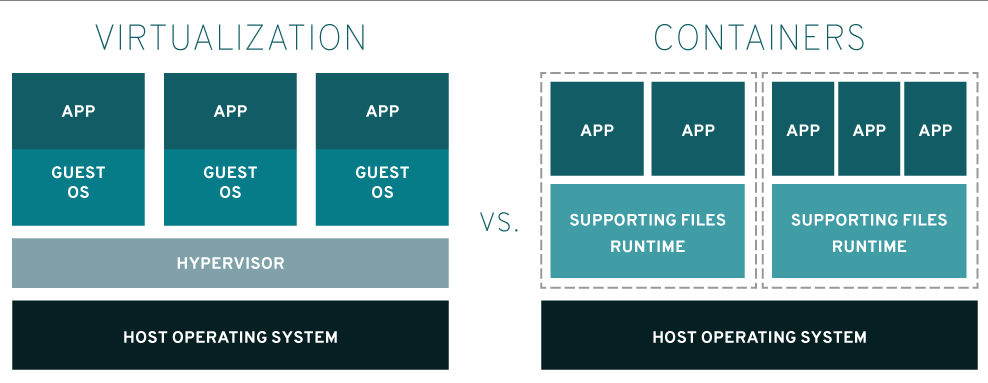
\includegraphics[scale=0.45]{Imagenes/dockervsvm1.png}
\caption{Virtualización vs Containers.}
\label{dock-1}
\end{figure}

Docker, en concreto, es una plataforma que mejora el sistema LXC (proyecto
de contenedores de linux) combinando este sistema con herramientas propias.
Actualmente se puede ejecutar tanto en Linux como en MAC o Windows, lo que
hace que cada contenedor pueda ser lanzado indistintamente de la máquina o
el SO. Pero, ¿esto es del todo cierto? ¿cómo puede lanzar un contenedor de
Linux en Windows o viceversa? Evidentemente, esto no es posible, en el caso
de Windows, por ejemplo, la solución consiste en lanzar una maquina virtual
con un kernel de Linux sobre el Hyper-V (el hypervisor de windows a partir
de Windows 10) o sobre una maquina virtual Virtualbox (versiones
anteriores) y ejecutar todos los contenedores de Linux sobre esa máquina
virtual. Sin embargo, los contenedores de Windows únicamente es posible
lanzarlos desde este mismo sistema operativo \cite{Dck-10}.

Cada imagen del contenedor Docker se almacenan físicamente en el disco con
una estructura de diferentes capas que hace que, cada imagen, sea aún más
ligera de almacenar. Dicha cuestión ocurre porque se puede aplicar algo
similar al concepto de herencia entre las diferentes máquinas permitiendo
así, que cada imagen sea a su vez parte de la máquina de la que hereda.
Para entender esto, debemos saber cuál es la estructura de un Dockerfile
que define la imagen de un contenedor Docker. Cada una de estas imágenes se
etiquetan con un nombre de modo que sean fáciles de manejar posteriormente.

Un Dockerfile es un fichero que contiene diferentes macros para compilar y
crear la imagen. La primera instrucción de dicha imagen siempre es el
contenedor base \cite{Dck-11}. Cada una de las instrucciones que se
ejecuten da lugar a una nueva capa (layer) que se almacena y se puede
compartir, si fuera necesario, entre otros contenedores. Por otra parte,
cada contenedor tiene un límite de capacidad, que en este caso es un límite
de capas para cada contenedor. Cuando se ha realizado este trabajo el
límite estaba en 150 capas. \cite{Dck-12}.

Este diseño de capas nos permite, además de ocupar menos espacio en disco,
poder tenerlas en un repositorio y solo descargarnos las capas que no
tenemos. Docker nos proporciona la herramienta Docker Hub, un repositorio
público similar a los repositorios de código pero que, a diferencia de
estos, almacena las imágenes de los contenedores. Además, podremos
descargar cualquier imagen y ejecutarla en cualquier máquina que tenga
instalado Docker.

Para finalizar, Docker nos ofrece la herramienta “compose”. Dicha
herramienta nos permite lanzar y administrar, con una sola instrucción,
diversas aplicaciones y servicios de múltiples contenedores. Para ello, se
define un fichero en formato YAML según la estructura definida por Docker
\cite{Dck-13}. Gracias a dicha herramienta, es muy sencillo levantar y
manejar toda una estructura de aplicaciones y diferentes servicios.



\section{Apache Kafka\label{Kafka}}

Apache Kafka surgió de la empresa LinkedIn a partir del sistema que tenían
para recopilar múltiples métricas de sus sistemas y aplicaciones. Tenían un
sistema que registraba la información de la actividad de cada usuario a
partir de diferentes XMLs con una cantidad indefinida de variables, lo que
lo hacía complejo y propenso a fallos. Para solucionar estas problemas se
realizaron diferentes estudios que llevaron a Linkedin a usar una
aplicación de gestión de mensajes, en concreto ActiveMQ. Cuando comenzaron
a usar ActiveMQ descubrieron que tenían una serie de necesidades
adicionales que dicho software no contemplaba. La imposibilidad de escalar
dicho software y una serie de fallos que descubrieron posteriormente cuando
estaban procesando sus datos, dio lugar a que LinkedIn realizará un
desarrollo propio. Dicho desarrollo fue bautizado como Kafka. Esta
herramienta debía reunir una serie de características para solventar los
problemas concretos de LinkedIn que con un sistema de gestión de mensajes
tradicional no bastaba. Necesitaban que tanto los productores como los
consumidores de los mensajes pudieran estar desacoplados a la hora de
insertar u obtener un mensaje. También necesitaban que los mensajes fueran
persistentes en las colas de mensajes de forma que los múltiples
consumidores pudieran hacer uso de los mensajes. A su vez, era necesario
optimizar al máximo el tiempo que se necesitaba en procesar los mensajes.
Por último, era importante que pudieran escalar el sistema horizontalmente
si es necesario por la cantidad de mensajes o por nuevos tipos de mensajes.
Finalmente, hemos de subrayar que Kafka está escrito en el lenguaje Scala y
se lanzó como proyecto Open Source y forma parte de la Apache Software
Foundation \cite{Kfk-1}. Para entender Kafka, debemos de tener en cuenta
que es una simple cola de mensajes en la que varios productores y
consumidores pueden estar a la vez enviando y recibiendo mensajes. Dado que
los mensajes de Kafka son persistentes, esto hace que se pueda ver como el
gran fichero de log de varias aplicaciones y que, posteriormente, otras
aplicaciones leen para aplicar a esos datos diferentes procesos
convirtiéndolos, por ejemplo, en estadísticas \cite{Kfk-6}. En el caso de
una arquitectura Lambda, por ejemplo, podemos leer de la misma cola tanto
para la \emph{Bach Layer} como para la \emph{Speed Layer} y esto quiere
decir que toda la información de que proviene de una cola se mantiene en un
mismo sistema sin necesidad de replicar datos.

Podemos diferenciar Kafka en las siguientes partes:

\textbf{Mensajes y lotes (batch)}: La forma en que se introduce y se saca
la información en Kafka es a través de mensajes. Cada mensaje, para Kafka,
es una serie de bytes sin significado alguno a excepción de la parte de
metadatos que contienen una clave y una marca de tiempo. La clave se puede
usar para distribuir los datos en diferentes particiones o para hacer un
seguimiento de los mensajes. Los mensajes se pueden escribir en lotes ({\em
  batch}), que no es otra cosa que una colección de mensajes. Eso nos
permite escribir y obtener los mensajes mucho más rápido, ya que podemos
escribir o recibir varios mensajes en una sola petición. Los mensajes se
mantienen persistentes hasta un tiempo definido o hasta que la cola llegue
a una cantidad fija de espacio, por ejemplo, 20 GB. Si se llega al límite
por espacio, se borrarán los primeros mensajes que llegaron a la cola, y si
llega al límite por tiempo se borrarán cuando haya pasado el tiempo de
caducidad del mensaje.

\textbf{Estructuras}: Aunque para Kafka los mensajes son únicamente bytes,
se recomienda usar algún tipo de estructura. Esto no es una propiedad de
Kafka como tal, pero es una recomendación muy útil. Las estructuras más
utilizadas sobre los mensajes de Kafka son JSON y XML.

\textbf{Topics y particiones}: Al igual que en una base de datos tenemos
tablas o en un sistema de ficheros tenemos directorio, Kafka organiza los
mensajes por topics. Estos topics, a su vez, se dividen en particiones
donde se almacenan los mensajes. Los mensajes se almacenan en orden de
llegada y cada partición puede estar en diferentes servidores. Además.
puede haber replicación en las particiones o no, según las necesidades. En
la figura \ref{Kfk-img-1} \cite{Kfk-2} podemos ver cómo se escriben los
mensajes de un topic en diferentes particiones. Además, a través de las
claves de los mensajes, podemos repartir los mismos entre las diferentes
particiones.


\begin{figure}[htp]
\centering
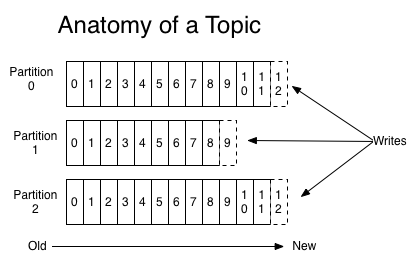
\includegraphics[scale=0.75]{Imagenes/kafka1.png}
\caption{Funcionamiento del Topic en Kafka con sus particiones.}
\label{Kfk-img-1}
\end{figure}

\textbf{Productores y consumidores}: Para Kafka, sus clientes, son los
diferentes usuarios del sistema que escriben o leen la información, es
decir, los productores y los consumidores. Los productores o publicadores
son los encargados de escribir los mensajes en un topic. Sin embargo, les
da lo mismo en qué partición se encuentre cada mensaje, por lo que será
Kafka el encargado de distribuir los mensajes en las diferentes
particiones. Opcionalmente los productores pueden añadir una clave al
mensaje y así poder repartir ellos mismos los mensajes entre las diferentes
particiones. A la misma vez, pueden haber varios productores escribiendo en
un mismo Topic. Los consumidores o lectores son los encargados de leer y
consumir el mensaje, con la característica de que el mensaje no se borrará
una vez leído si no, como hemos dicho, según la caducidad del mismo. Cada
uno de los consumidores se suscribe a un tema he irá leyendo los mensajes
en el orden en el que se han producido. Además, puede haber varios
consumidores leyendo de un mismo topic y de una misma partición. Los
consumidores pueden leer desde el principio de la cola o empezar con un
desplazamiento u offset específico. Una vez vaya leyendo los mensajes, el
consumidor sabrá por cuál se ha quedado y podrá seguir leyendo a partir del
siguiente mensaje. Esto significa que los consumidores pueden detenerse o
reiniciarse y sabrán volver al punto por donde se habían quedado. También
existen grupos de consumidores que leen, cada uno, una parte de la cola, de
forma que pueden ir procesando, cada uno, una parte del tema. Estos grupos
de consumidores también son tolerantes a fallos ya que, si alguno deja de
consumir, automáticamente, los demás se irán equilibrando para que no se
pierdan mensajes. Por último decir que, a un consumidor de un grupo se le
puede asignar una partición de forma que sea a ese consumidor el que lee,
mayormente, dicha partición. Decimos mayormente porque si hay un fallo por
parte de otro consumidor, para que una partición no se quede sin leer,
automáticamente se le asignará mensajes de otras particiones para que los
procese. Podemos ver como un grupo de consumidores consumen un topic en la
figura \ref{Kfk-img-2} \cite{Kfk-1}.

\begin{figure}[htp]
\centering
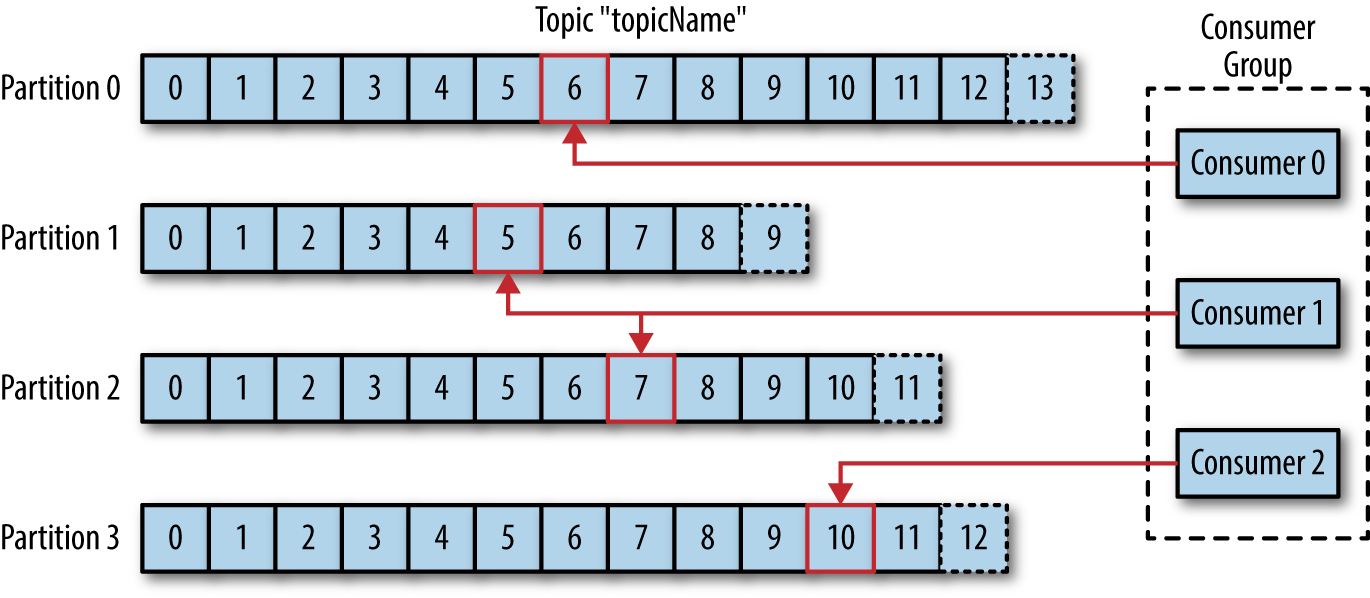
\includegraphics[scale=0.30]{Imagenes/kafka2.png}
\caption{Distribución del trabajo entre consumidores de un Topic Kafka.}
\label{Kfk-img-2}
\end{figure}

\textbf{Brokers y Clusters}: Cada servidor con Kafka se le llama {\em
  broker} y es el encargado de recibir y enviar los mensajes desde los
productores a los consumidores. Como ya sabemos, una vez recibe un mensaje,
estos deben permanecer en disco, esto lo hace el broker asignándole el
offset correspondiente y eliminando los mensajes que han caducado. El
broker también es el encargado de gestionar las diferentes particiones
siendo capaz de manejar miles de particiones y millones de mensajes,
dependiendo del hardware donde resida. Un broker está diseñado para formar
parte de un cluster junto a más brokers, los cuales son gestionados a
través de Zookeeper. Mediante este mismo, se gestiona quién será el líder
del cluster, encargado de repartir las particiones, controlar la
replicación de datos y revisar fallos. Si el líder falla, será Zookeeper el
encargado de asignar un nuevo líder.


\section{Apache Hadoop\label{Hadoop}}

Obviamente, cuando hablamos de Big Data tenemos que hacer referencia a
Apache Hadoop. Para la realización de esta herramienta, se basaron en dos
artículos publicados por Google sobre su sistema de ficheros distribuido
\cite{Hdp-2} y MapReduce \cite{Hdp-3}. El sistema de ficheros de Hadoop fué
bautizado como HDFS convirtiéndose en una herramienta muy popular de la que
hacen uso grandes empresas como Yahoo!, Last.fm, Facebook o el New York
Times. Además de esto, en 2009, Hadoop superó el récord de Google en
ordenar un terabyte de datos en menos tiempo \cite{Hdp-1}. Por otro lado,
Apache Hadoop forma parte de Apache Foundation, lo que quiere decir que es
totalmente OpenSource.

Actualmente, la arquitectura de la versión 3 de Hadoop, está formada por
cuatro módulos principales y sus diferentes servicios \cite{Hdp-4}:

\begin{itemize}
\item \textbf{Hadoop Common}: Este paquete contiene las utilidades comunes
  que soportan todos los demás módulos de Hadoop.
\item \textbf{Hadoop Distributed File System (HDFS)}: Es el sistema de
  ficheros distribuido de Hadoop. Por definición es un sistema de ficheros
  distribuidos que proporciona un alto rendimiento a los datos de
  aplicación. Tiene una estructura maestro/esclavo que se compone de los
  siguientes servicios:
  \begin{itemize}
  \item \textbf{Namenode}: Administra el espacio de nombres del sistema de
    ficheros y regula el acceso a los diferentes ficheros. Además, asigna
    el datanode donde se almacenará cada bloque físico de cada fichero para
    que quede balanceado dicho sistema. Por tanto, en este nodo se
    encontrarán los metadatos de donde se encuentra cada bloque.
  \item \textbf{Datanode}: Es un nodo de almacenamiento. En dicho nodo
    existirán bloques de datos, asignados por el NameNode.
  \item \textbf{Secondary NameNode}: Es una réplica del namenode que se usa
    como copia por si en algún momento el NameNode cae. Se hace una copia
    de los metadatos cada hora o cada millón de transacciones por defecto.
  \item \textbf{Checkpoint node}: Al igual que el Secundary NameNode, hace
    copias de seguridad del NameNode, sin embargo, este nodo no tiene la
    capacidad de sustituirlo.
  \end{itemize}
\item \textbf{Hadoop YARN}: Este módulo es el framework que gestiona los
  trabajos y los diferentes recursos del cluster. La idea consiste en
  separar la planificación y la supervisión de los diferentes trabajos
  sobre Hadoop. También usa una estructura de maestro/esclavo para los
  cuales se suministran los siguientes servicios:
  \begin{itemize}
  \item \textbf{Resource Manager}: Este servicio se considera el “maestro”.
    Tiene dos funcionalidades principales, la función de Scheduler
    (planificador) y la función de ApplicationsManager (gestor de
    aplicaciones). Como planificador debe ser capaz de asignar los recursos
    necesarios a cada aplicación cuando lo necesite o reiniciar una
    aplicación en caso de fallo. Como gestor de aplicaciones es el
    encargado de asignar trabajo a cada uno de los componentes del cluster.
  \item \textbf{Node Manager}:Es el responsable de iniciar y administrar
    los trabajos para una nodo del cluster.
  \item \textbf{ProxyServer}: Por defecto, se ejecuta junto al Resource
    Manager, pero se puede ejecutar por separado. Se encarga de reducir
    ataques web que puedan producirse a través de YARN.
  \end{itemize}
\item \textbf{Hadoop MapReduce}: Es el módulo para el procesamiento
  paralelo de grandes conjuntos de datos. Este sistema está basado en YARN.
  Además, tiene un servicio adicional que podemos añadir:
  \begin{itemize}
  \item \textbf{HistoryServer}: simplemente muestra a través de una web los
    logs que producen los diferentes trabajos de MapReduce.
  \end{itemize}
\end{itemize}

HDFS, como ya hemos dicho, es el sistema de ficheros de Hadoop, cuya
característica más importante es que es distribuido, aunque no es la única
característica que posee. HDFS, como los sistemas de ficheros
convencionales, distribuye los diferentes ficheros en bloques de un tamaño
fijo, normalmente de 128 MB, ya que suponen ficheros de gran tamaño, aunque
esto es modificable. Dichos bloques están divididos entre los diferentes
nodos del cluster de forma que sea más fácil realizar diversos tratamientos
sobre ellos de forma paralela. Además de esto, contamos con la replicación
de los distintos bloques, según establezcamos cuantas replicaciones de
bloque queramos. Esto tiene muchas implicaciones tales como cuando cae uno
de los nodos, siempre tenemos los datos disponibles en otro nodo, si uno de
los nodos cae o se rompe el disco duro, podemos volver a generar dicho nodo
a partir de los metadatos del namenode y la replicación de bloques. Dicho
esto, podemos ver que no tiene sentido montar un RAID sobre el servidor, ya
que el sistema de Hadoop te proporciona dicha funcionalidad.

MapReduce consiste en uno o varios procesos distribuidos que manejan
grandes volúmenes de datos. Tiene dos funciones principales, Map y Reduce.
La función Map genera una tupla clave/valor intermedios y la función Reduce
combina esos valores para cada clave para obtener un resultado. Dicho esto,
se muestra en la figura \ref{hdImg1} \cite{Hdp-1} un ejemplo de cómo
funcionaria gráficamente:

\begin{figure}[htp]
\centering
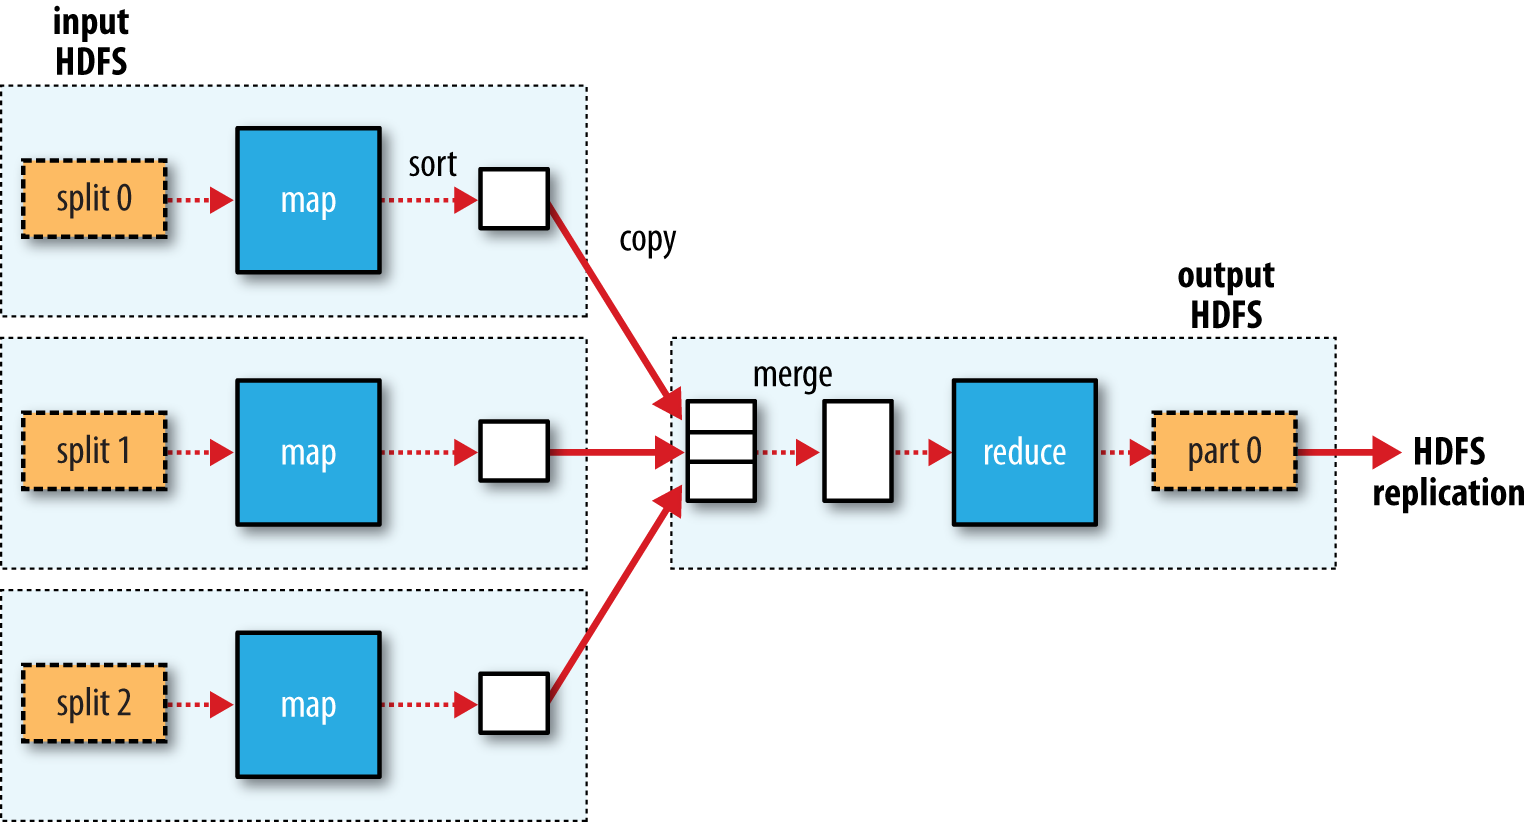
\includegraphics[scale=0.28]{Imagenes/hadoop1.png}
\caption{Funcionamiento de MapReduce sobre HDFS.}
\label{hdImg1}
\end{figure}

Por último, decir que Apache Hadoop está programado en Java y necesitamos
la JVM (Java Virtual Machine) para ejecutarlo.


\section{MongoDB\label{MongoDB}}

MongoDB es una base de datos NoSQL en concreto, de tipo documental.
Almacena los datos con una estructura muy parecida al JSON llamada BSON.
MongoDB es código abierto, lo que quiere decir que cualquiera puede
reportar fallos directamente del código o contribuir a nuevas mejoras, lo
que finalmente ha contribuido a su popularidad.

Dado que MongoDB fue diseñada para la web moderna \cite{Mng-2}, está
pensada para tener gran flujo de entrada y salida de datos, con un esquema
dinámico. Esto quiere decir que, frente al SQL tradicional, podemos
insertar y extraer datos sin tener que definir previamente una estructura
fija. Al almacenar BSON podemos añadir todos los tipos de datos que
queramos y que nos permita JSON, por tanto tenemos arrays o documentos
dentro de documentos entre otros tipos de datos. Estas bases de datos son
formadas por colecciones que a su vez, contienen los diferentes documentos.
Cada uno de estos documentos contiene múltiples campos los cuales, definen
las claves por las que realizar las búsquedas posteriormente. Podemos ver
esto último en la figura \ref{Mng-img-1} \cite{Mng-5}. Esto hace que las
búsquedas sean realmente potentes ya que son muy flexibles y lo
sorprendente es que son en algunos casos, incluso más rápidas que muchas
bases de datos SQL tradicionales ya que, no hace falta hacer tantos JOINs.
Otra diferencia entre las bases de datos NoSQL y una SQL relacional es que
no soporta transacciones, por lo que no es recomendable usar MongoDB en
programas de tipo transaccionales. Por otra parte, una de las
características importantes de MongoDB para este proyecto es que nos
permitirá realizar consultas y operaciones de tipo geoespaciales
\cite{Mng-3}.


\begin{figure}[htp]
\centering
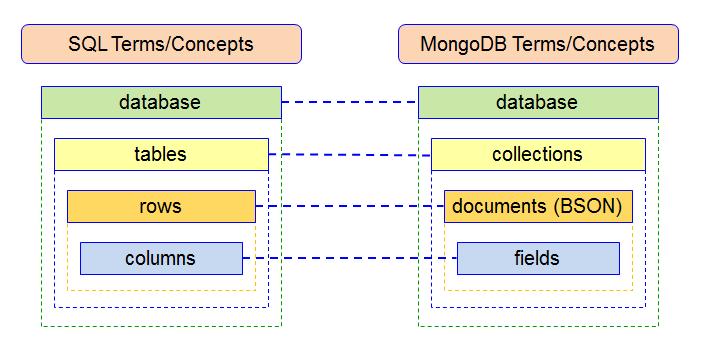
\includegraphics[scale=0.57]{Imagenes/mongo1.png}
\caption{Relación de conceptos de SQL a MongoDB.}
\label{Mng-img-1}
\end{figure}


Otra de las características que hacen a MongoDB tan potente es el hecho de
que es fácilmente escalable \cite{Mng-1}. Podemos crear réplicas o
distribuir los datos horizontalmente de una forma fácil. Para distribuir
los datos, MongoDB añade el concepto de sharding, que consiste en una
colección distribuida a través de un hash de los campos obligatorios que
tengan los documentos de dicha colección, como puede ser el id. Por otro
lado, también tenemos las réplicas, nombradas Replica Set. El Replica Set
consiste en tener un servidor primario y uno o varios secundarios.
Normalmente se hacen todas las peticiones al servidor primario y es el que
se encarga de que los secundarios se mantengan actualizados. Dependiendo de
la carga podemos hacer que se puedan realizar consultas a los secundarios
pero las peticiones van al servidor primario por normal general. Si el
servidor primario cae, se asignará automáticamente a otro servidor la
función de primario hasta que el primario se recupere. Con las librerías de
MongoDB esto se hace totalmente transparente al programador por lo que, una
vez montadas las réplicas o los shards, el programador hará las lecturas y
escrituras tal y como lo haría si solo existiera un único servidor de
MongoDB.

\section{Apache Spark\label{Spark}}

Apache Spark surge de las problemáticas de usar Hadoop en plataformas
generales, específicamente cuando hablamos de algoritmos de aprendizaje
automático en las que se necesitaban realizar múltiples iteraciones sobre
los mismos datos. El equipo de Spark diseñó un API basada en la
programación funcional, en concreto usaron el lenguaje Scala que permitía,
en un solo trabajo, realizar varias interacciones de MapReduce
\cite{Spk-1}. Apache Spark lanzó la versión 1.0 en 2014 y Spark 2.0 en
2016, realizando regularmente nuevas aportaciones al proyecto \cite{Spk-2}.
Actualmente está disponible la versión 2.3, que usaremos en este trabajo. A
continuación hablaremos de los aspecto s más importantes de este framework.

Una de las características más importantes de cómo funciona Spark es como
distribuye el trabajo. Spark soporta un flujo de datos acíclico creando un
\textbf{DAG} (Directed Acyclic Graph) de etapas de trabajo que, por
definición del mismo, es un grafo de trabajo sin ciclos \cite{Spk-5}. Esto
nos permitirá repartir las tareas de trabajo entre los distintos nodos del
cluster y favorecer la recursión dentro del mismo. Para poder añadir
trabajos a este DAG podemos hacerlo a través de la variable Spark Context.
Cuando añadimos un trabajo al Spark Context, Spark reorganiza el DAG y
optimiza la gestión de las tareas añadidas. Por otro lado, la siguiente
característica más importante de Spark son los \textbf{RDD} ({\em Resilient
  Distributed Dataset}) que consiste en una colección inmutable de datos
particionada con la que se puede operar de forma paralela. Sobre estos RDD
podemos realizar diferentes operaciones como MapReduce o cualquiera que nos
permitan los módulos de Spark \cite{Spk-4}.

En cuanto a la arquitectura de un cluster de Spark, tenemos dos tipos de
nodos principales. El más importante es el \textbf{nodo master}, que es el
que coordina a los demás nodos. Este nodo dirige a los \textbf{nodos
  esclavos} (o slaves) que son los que ejecutan los trabajos de Spark.
Además de estos nodos, podemos añadir un servicio de monitorización de
trabajos que se llama \textbf{history-server}. Finalmente, como se ha
explicado, podemos ver cómo se comunican y distribuyen los trabajos en la
figura \ref{SpkImg-1} \cite{Spk-6}. Aunque tengamos esta estructura,
también podremos integrar Spark con un clúster de Hadoop sin realizar
grandes modificaciones. Para integrar el clúster simplemente tendremos que
añadir las librerías de Spark al HDFS y lanzar los trabajos desde un nodo
que contenga Spark, esto hace que Spark esté siendo tan famoso ya que
puedes reutilizar la estructura si existiera manteniendo ambos framework.

\begin{figure}[htp]
\centering
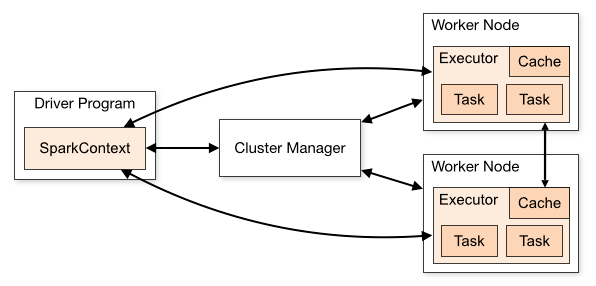
\includegraphics[scale=0.65]{Imagenes/spark1.png}
\caption{Comunicación en los nodos de Apache Spark para la realización de
  trabajos.}
\label{SpkImg-1}
\end{figure}

Por último, Spark se divide entre diferentes módulos que nos facilitará
diferentes operaciones sobre los datos \cite{Spk-3}:

\begin{itemize}
\item \textbf{Spark Core Engine}: Es el módulo principal de Spark. Sobre
  este módulo se ejecutan todos los demás. Permite la persistencia en
  memoria de forma que permita una gran velocidad al pedir datos.
\item \textbf{Spark Sql y DataFrames}: Este módulo nos permite trabajar a
  Spark con datos estructurados. Sobre estos datos podemos realizar
  consultas SQL.
\item \textbf{Spark Streaming}: Este módulo nos permite trabajar con {\em
    microbaching}, creando aplicaciones escalables y tolerantes a fallos.
\item \textbf{MLlib}: Este módulo es el que contiene los diferentes
  algoritmos de aprendizaje automático que podemos usar con Spark.
\item \textbf{GraphX}: Este módulo nos permitirá realizar procesamiento de
  gráficos en paralelo. En definitiva, con este módulo, tenemos una serie
  de operaciones sobre grafos que nos permite manejar los mismos de una
  forma rápida y escalable.
\item \textbf{SparkR}: Este módulo proporciona una interfaz ligera de R que
  implementa las diferentes operaciones distribuidas que se aplican sobre
  los RDDs de Spark.
\end{itemize}

A partir de aquí podemos ver toda la funcionalidad que nos aporta Spark
frente a Hadoop \cite{Spk-7}. Por otro lado, al igual que con Hadoop,
tenemos varios lenguajes con los que programar los diferentes trabajos. En
nuestro caso usaremos Python, pero podríamos usar R o Java. También
podríamos usar otros lenguajes como C\# a partir de diferentes módulos que
están a disposición en la página oficial de Spark \cite{Spk-6}.


\section{Elastic\label{Elastic}}

Elasticsearch es un motor de búsqueda y recuperación de documentos de
código abierto construido sobre Apache Lucene. En torno a este motor, se ha
formado la empresa Elastic que promociona Elasticsearch junto a su stack de
tecnologías, aportando a diferentes empresas un sistema de búsqueda en
tiempo real avanzado y versátil \cite{Elk-1}.

Actualmente podemos definir Elasticsearch como un motor de búsqueda y
análisis de texto, con una interfaz RESTful, compatible con múltiples
usuarios y capaz de almacenar grandes cantidades de datos. Junto con este
motor encontramos Elastic Stack, una serie de tecnologías que permiten
conectarte a Elasticsearch de una forma más segura y sencilla, tanto para
escribir como para leer datos.

Elastic Stack tiene como núcleo Elasticsearch y está formado por Kibana,
Logstash, Beats, ECE y X-Pack. Cada uno de estos módulos son totalmente
independientes e interoperables unos con otros. A continuación, explicamos
cada uno de ellos \cite{Elk-4}:

\begin{itemize}
\item \textbf{Elasticsearch}: Considerado el corazón de Elastic Stack, se
  trata del motor de búsquedas basado en Apache Lucene. Se pueden insertar
  documentos de tipo JSON y hacer analiticas o busquedas sobre ellos. Para
  realizar las inserciones, las modificaciones y las consultas hay que usar
  una API RESTful con diferentes operaciones tipo GET, PUSH, PUT o DELETE,
  acompañadas de un JSON con las operaciones a realizar. Los documentos en
  Elasticsearch se introducen en un índice, con un tipo y un identificador
  para facilitar la búsqueda y reconocer más fácilmente los distintos
  campos del documento. Otra característica importante es que, aunque
  definas un tipo en Elasticsearch, siempre puedes añadir un documento con
  otros campos. Finalmente, para acceder al documento podemos hacerlo desde
  cualquier navegador realizando las consultas de la siguiente forma:
  servidorElasticsearch:PORT/indice/tipo/identificador y nos devolverá el
  objeto JSON que pedimos.
\item \textbf{Beats}: Este módulo puede enviar datos de diferentes fuentes,
  principalmente de ficheros, aunque también puede leer de bases de datos
  o, simplemente, leer las métricas que te aporta el sistema operativo
  sobre el hardware. Estos datos son enviados a Logstash o a Elasticsearch
  sin ningún tipo de procesado previo. Se define como un agente y está
  escrito en Go.
\item \textbf{Logstash}: Se trata de un sistema de procesamiento
  distribuido el cual obtiene datos de diferentes fuentes para insertarlos
  en otras, normalmente en Elasticsearch. Cuando hablamos de Logstash
  hablamos de un servicio con una o varias pipelines (tuberías). Cada
  pipeline tiene tres fases. La primera obtendrá los datos de cualquier
  tipo de fuente (entrada), la segunda filtra y procesa los datos y la
  tercera inserta los datos en Elasticsearch o cualquier otra salida.
\item \textbf{Kibana}: Se trata de un componente que se conecta
  directamente con Elasticsearch que te permite manejar y visualizar la
  información. Te permite establecer diferentes métricas en tiempo real e
  ir explorando los diferentes datos que se van insertando en
  Elasticsearch. Además de crear diferentes gráficas también permite crear
  Dashboards. Para acceder a Kibana se debe hacer vía web donde podrás
  manejar y administrar el componente.
\item \textbf{ECE (Elastic Cloud Enterprise)}: Sirve para administrar tanto
  Kibana como Elasticsearch desde un mismo punto. Gracias a este módulo
  podemos monitorear y administrar un cloud de Elastic Stack desde un solo
  punto vía web o vía consola. También tiene una modalidad en la cual
  puedes montar directamente Elastic sobre un servidor de Azure o AWS.
\item \textbf{X-Pack}: Realmente esto no es un módulo como tal, sino una
  serie de features. Simplemente se trata de todos los componentes extras
  que están bajo licencia y son de pago. X-Pack se compone de:
\begin{itemize}
\item \textbf{Security}: Nos permite tener active directory, LDAP o bien,
  mantener la información cifrada en Elasticsearch.
\item \textbf{Alerting}: Nos permite recuperar información de Elasticsearch
  y poner alertas como que salte la alerta cuando se suma determinado valor
  de una variable en un mes. Las alertas se pueden transmitir por
  diferentes medios como por slack o email.
\item \textbf{Monitoring}: Nos permite ver el estado del cluster.
\item \textbf{Reporting}: Nos permite crear Reports a través de Kibana.
\item \textbf{Graph}: Nos permite ver diferentes conexiones entre los
  documentos de una forma gráfica.
\item \textbf{Machine Learning}: Nos permite ejecutar diferentes algoritmos
  de machine learning sobre Elasticsearch.
\item\textbf{ Elasticsearch SQL}: Nos permite hacer consultas sobre
  Elasticsearch con una sintaxis SQL.
\end{itemize}
\end{itemize}

Sobre cualquiera de los módulos se pueden instalar diferentes plugins o
librerías para añadir seguridad, conectores, operaciones o incluso
gráficos. Esta es una de las razones por la que Elastic Stack es tan
popular ya que, al ser código libre, todo el mundo puede aportar su granito
de arena, mejorar las herramientas o crear nuevos plugins. Actualmente,
estamos en la versión 6.


%%% Local variables:
%%% TeX-master: "main.tex"
%%% coding: utf-8
%%% ispell-local-dictionary: "spanish"
%%% TeX-parse-self: t
%%% TeX-auto-save: t
%%% fill-column: 75
%%% End:
